\documentclass{amsart}

\usepackage{amsmath, amsthm, amssymb} %AMS math

\usepackage{graphicx}% Include figure files
\usepackage{bm}% bold math
\usepackage{color} % colored text
\usepackage[pdftex,colorlinks=true,
allcolors=blue
]{hyperref}% add hypertext capabilities
\usepackage{paralist}% for compactitem used by Marko
\usepackage{multirow}% multicolumn/row cells in tables

\usepackage{url} % add auto-linked urls
\usepackage{mathtools} % shortintertext, and other useful math-related features
\usepackage{siunitx}
\sisetup{per-mode = symbol}
\usepackage[dvipsnames]{xcolor}
\usepackage{listings} % including code
\usepackage{amsrefs} % references

\graphicspath{{figs/}} % store figures in figs subfolder

% packages for plotting directly in MATLAB
\usepackage{pgfplots}
\pgfplotsset{compat=newest}


%% comments
\newcommand{\marko}[1]{\textcolor{red}{(MB: {\bfseries #1})}}
\newcommand{\yourname}[1]{\textcolor{red}{(STUDENT: {\bfseries #1})}}

\begin{document}

\title{Title of our paper}

\author{First Last}
\address{Department of Mathematics, Clarkson University,
Potsdam, NY}
\email{email@clarkson.edu}

\author{Marko Budi\v{s}i\'c}
\address{Department of Mathematics, Clarkson University,
Potsdam, NY}
\email{mbudisic@clarkson.edu}
\urladdr{http://people.clarkson.edu/~mbudisic} % Delete if not wanted.

\begin{abstract}
Great stuff.
\end{abstract}

\maketitle % typeset the title page
\tableofcontents % table of contents

\section{Introduction}

\begin{itemize}
\item motivation for the problem
\item discussion of existing results in literature, covering all aspects of the paper
\item announcement of the original contribution
\item short outline of the paper sections (Section 1 does this, Section 2 does that, etc.)
\end{itemize}

\section{Problem description}

\section{Main technique}

\subsection{Theory}

\subsection{Implementation}

\section{Results}

\section{Discussion and Conclusions}

\bibliography{bibliography} % bibliography.bib stores references

\clearpage \appendix

\section{How to use LaTeX?}

\subsection{General advice}

\textbf{  All the help you need is found here: \url{https://en.wikibooks.org/wiki/LaTeX}. }

You can create a bulleted list
\begin{itemize}
\item First
\item Second
\item Third
\end{itemize}

You can also enumerate
\begin{enumerate}
\item First
\item Second
\item Third
\end{enumerate}

If you want a tighter itemization, use \verb|compactitem| and \verb|compactenum|
\begin{compactitem}
\item First
\item Second
\item Third
\end{compactitem}

\begin{compactenum}
\item First
\item Second
\item Third
\end{compactenum}

\subsection{Mathematics}
Some math $\int_0^Tx(t)dt$. If you'd like to put an equation in its own line, this is how you do it:
\begin{equation}
x(t) = x_0 + \int_0^T f(x(\tau))d\tau  \label{eq:ode-solution}
\end{equation}


You can also refer to an equation that you made, if you gave it a label, just like this \eqref{eq:ode-solution}.


Most people get matrices wrong (overly complicated) in \LaTeX. This is the right way:
\[ %this produces unenumerated equation.
  \begin{bmatrix}
    1 & 2 \\
    \ast & 3
  \end{bmatrix}
\]
More details are here:
\url{https://en.wikibooks.org/wiki/LaTeX/Mathematics\#Matrices_and_arrays}.

\subsection{Graphs directly in \LaTeX}

If you want to include an image, this is how you do it. And you can also refer to the Figure~\ref{fig:graph}.
\begin{figure}
  \centering
  \includegraphics[width=0.2\linewidth]{figs/graph.png}
  \caption{This is a graph.}\label{fig:graph}
\end{figure}

LaTeX (with help of pgfplot) can also create graphs of functions.
\begin{figure}[htb]\centering
   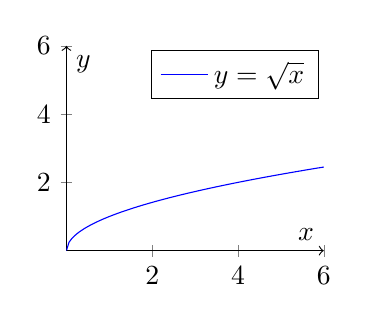
\begin{tikzpicture}
     \begin{axis}[
       xmin=0, xmax=6,
       xlabel={$x$},
       ymin=0, ymax=6,
       ylabel={$y$},
       axis lines=middle,
       axis line style=->,
       width=.4\textwidth
     ]
       \addplot[no marks,blue,-,domain=0:6, samples=100] expression{sqrt(x)};
       \addlegendentry{$y=\sqrt{x}$};
     \end{axis}
   \end{tikzpicture}
 \end{figure}
 
 Figure~\ref{fig:csvfig} was made purely in \LaTeX.\footnote{For more such plots see \url{http://pgfplots.sourceforge.net/gallery.html}}

\begin{figure}[htb]
  \centering
  \begin{tikzpicture}
\begin{axis}[width=0.8\linewidth, height=0.55\linewidth,
  enlargelimits=0.15,
  xmin=-5,xmax=5, mark size=1.5pt,
  legend pos = north west, legend style={fill=none,draw=none},
  yticklabel style={/pgf/number format/.cd,fixed,precision=2},
  xlabel={Value}, ylabel={Proportion} % labels
  ]
  \addplot+ table[x=Value, y=Proportion, col sep=comma]{figs/dataset.csv};
\end{axis}
\end{tikzpicture}
\caption{Graph made directly in LaTeX.}\label{fig:csvfig}
\end{figure}

 \subsection{Syntax-highlighted code}
 This is how you include some code\footnote{For more see \url{https://www.overleaf.com/learn/latex/Code_listing\#Using_listings_to_highlight_code}.}:
\begin{lstlisting}[language=Matlab]
for k = 2:9
    u[k] = u[k-1] - 2*u[k] + u[k+1];
end
\end{lstlisting}

\subsection{Citing papers}

References are stored in \texttt{.bib} files. Instead of writing the bib file manually, it's best to install JabRef \url{http://www.jabref.org/} , BibDesk or another reference manager to edit the file.

To include a citation, enter \verb|\cite{Hill1894}| where Hill1894 is the paper label designated in the bib file.


 \subsection{Some \textbf{important formatting tips}:}
 \begin{compactitem}
 \item \textbf{Each sentence on its own line.} This helps with version control. LaTeX will ignore a single line-break and format sentences into a single paragraph. (Double line break leaves an empty line in your code, and LaTeX will start a new paragraph.)
\item Please make sure to use operator notation (with backslashes) when appropriate.\footnote{\url{https://en.wikibooks.org/wiki/LaTeX/Mathematics\#Operators}}
\item There's a lot of bad advice on how to write matrices. Here's the correct way: \url{https://en.wikibooks.org/wiki/LaTeX/Mathematics\#Matrices_and_arrays}
\item Mixing text and equations is another sore spot: \url{https://en.wikibooks.org/wiki/LaTeX/Mathematics\#Adding_text_to_equations}
\item Tidy multiline equations (use \verb|align| instead of \verb|eqnarray|)\footnote{This is an official guidance from TeX community \url{https://texfaq.org/FAQ-eqnarray}} \url{https://en.wikibooks.org/wiki/LaTeX/Advanced_Mathematics\#align_and_align.2A}
\item Annotating parts of equations using braces \url{https://en.wikibooks.org/wiki/LaTeX/Advanced_Mathematics\#Above_and_below}
\item Never use manual linebreak \verb|\\| in text (outside \verb|align|,\verb|bmatrix| and other similar multiline formula environments). If you think you need it, you're wrong.\footnote{\url{https://en.wikibooks.org/wiki/LaTeX/Paragraph_Formatting\#Manual_breaks}} Instead use an empty line (to break a paragraph), or displayed equations using a pair of \verb|$$| or \verb|\[|,\verb|\]| (preferred).
\end{compactitem}



\end{document}
